%% =============================================================================
%% HOW WELL DOES IT WORK?
%% =============================================================================

\section{How well does it work?} \label{sec:evaluation}

This section evaluates how well the LLM selects the right tool with the
right parameters. Numerical correctness of the underlying \proglang{Rust}
implementations is validated separately in
Appendix~\ref{app:numerical-validation}.

%% -----------------------------------------------------------------------------
\subsection{Tool selection evaluation}

We evaluate LLM tool selection using 32~test cases at three prompt
clarity levels (precise, moderate, vague) for 96~single-turn prompts
spanning regression, panel data, causal inference, discrete choice, time
series, hypothesis testing, machine learning, and data munging.  An
automated evaluation harness drives the live \pkg{prompt2analytics} HTTP
backend: it loads synthetic datasets with known data-generating
processes, sends each prompt, and scores complete responses on four
dimensions---tool selection, parameter extraction, numerical correctness,
and interpretation quality---each on a 0--2 scale.  A prompt is
classified as \emph{adequate} if it achieves $\geq 62.5\%$ of the
applicable maximum (5/8 for numeric tasks, 4/6 when numerical
correctness is N/A).  Tool definitions are auto-generated from the MCP
router's \code{JsonSchema} derives (119~Tier-1 tools), ensuring the LLM
sees the same parameter names and types as the server expects.

All evaluations used temperature~$= 0$ for deterministic output.
The evaluation harness, all 96~prompts (\code{test\_cases.json}),
dataset generators, and scoring data are provided in the supplementary
materials,\footnote{\url{https://github.com/umatter/prompt2analytics/tree/main/paper/code/e2e_eval}} enabling independent
verification and re-scoring.

\noindent Table~\ref{tab:model-results} lists the six models evaluated,
spanning frontier cloud, efficient cloud, and open-source deployment
scenarios, together with their single-turn adequate rates.
All models were accessed through cloud APIs (Anthropic,
OpenAI, or OpenRouter).  API-served models may change over time, so
exact replication of cloud-hosted results may not be possible; results
for proprietary models (Claude, GPT, Gemini) should be treated as a
snapshot.  For open-source models (Llama, Mistral), exact reproduction
is possible by serving fixed weights locally via Ollama.

\begin{table}[htbp]
\centering
\begin{threeparttable}
\caption{Models evaluated and single-turn adequate rates}
\label{tab:model-results}
\small
\begin{tabular}{lllr}
\toprule
Model & Version ID & Parameters & Adequate (\%) \\
\midrule
GPT-4.1 Mini & \code{openai/gpt-4.1-mini} & --- & 90.6 \\
Sonnet 4.6 & \code{claude-sonnet-4-6} & --- & 84.4 \\
Haiku 4.5 & \code{claude-haiku-4-5-20251001} & --- & 81.2 \\
Ministral 3B & \code{mistralai/ministral-3b-2512} & 3B & 80.2 \\
Gemini 2.5 Flash & \code{google/gemini-2.5-flash} & --- & 75.0 \\
Llama 4 Scout & \code{meta-llama/llama-4-scout} & 109B (17B active) & 50.0 \\
\bottomrule
\end{tabular}
\begin{tablenotes}[flushleft]
\item \emph{Note:} 96~single-turn prompts (32~test cases $\times$
3~clarity levels), temperature~$= 0$. Accessed March~2026.
Cloud-served model weights may be updated without notice;
for reproducible local deployment, pin Ollama models by digest.
Parameter counts marked ``---'' are not publicly disclosed.
\end{tablenotes}
\end{threeparttable}
\end{table}



The results demonstrate that tool selection---unlike code generation---is
achievable even by smaller models.  GPT-4.1~Mini achieves the highest
adequate rate (90.6\%), followed closely by Claude Sonnet~4.6 (84.4\%)
and Haiku~4.5 (81.2\%).  Notably, Ministral~3B, a 3B-parameter model
small enough to run on consumer hardware with only 6~GB VRAM, achieves
80.2\%---within 4~percentage points of Sonnet~4.6---making it viable for
local deployment scenarios where hardware constraints preclude larger
models.

\begin{figure}[htbp]
\centering
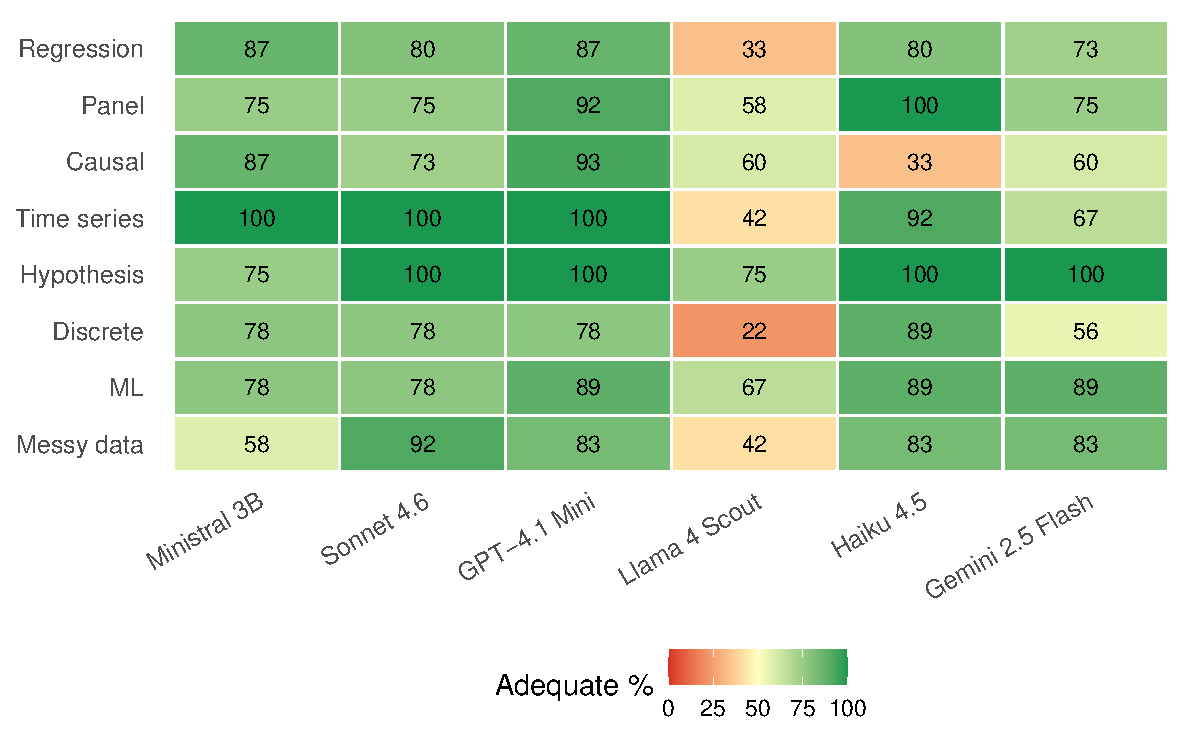
\includegraphics[width=0.95\textwidth]{figures/e2e_category_heatmap}
\caption{Adequate rate by test category and model (red = low,
green = high).  Errors concentrate in ambiguous method selection
(causal inference, discrete choice).}
\label{fig:accuracy-category}
\end{figure}

Figure~\ref{fig:accuracy-category} shows adequate rates by category.
Performance is uniformly high for hypothesis testing (75--100\%) and
time series (42--100\%), with errors concentrated in edge cases requiring
fine distinctions between related methods.  Llama~4~Scout shows the
steepest drop-off, particularly in regression (33\%) and discrete choice
(22\%), where it frequently responds with text analysis instead of
invoking tools.  Causal inference shows the widest variation across
models (33--93\%).  Appendix~\ref{app:e2e-eval} provides per-category breakdowns
for all six models.

Table~\ref{tab:e2e-results} breaks down the single-turn evaluation
by prompt clarity level.  Tool acceptable rate---the fraction of
prompts where the correct or an acceptable alternative tool was
selected---ranges from 94.8\% (GPT-4.1~Mini) to 52.1\%
(Llama~4~Scout).

\begin{table}[htbp]
\centering
\begin{threeparttable}
\caption{Single-turn evaluation by prompt clarity (96 prompts per model)}
\label{tab:e2e-results}
\small
\begin{tabular}{lrrrrr}
\toprule
 & Adequate & Tool & \multicolumn{3}{c}{Adequate by clarity} \\
\cmidrule(lr){4-6}
Model & rate (\%) & accept.\ (\%) & Precise & Moderate & Vague \\
\midrule
GPT-4.1 Mini       & 90.6 & 94.8 & 96.9 & 100.0 & 75.0 \\
Claude Sonnet 4.6  & 84.4 & 93.8 & 90.6 & 87.5 & 75.0 \\
Claude Haiku 4.5   & 81.2 & 83.3 & 90.6 & 90.6 & 62.5 \\
Ministral 3B       & 80.2 & 90.6 & 90.6 & 78.1 & 71.9 \\
Gemini 2.5 Flash   & 75.0 & 78.1 & 90.6 & 68.8 & 65.6 \\
Llama 4 Scout      & 50.0 & 52.1 & 59.4 & 46.9 & 43.8 \\
\bottomrule
\end{tabular}
\begin{tablenotes}[flushleft]
\item \emph{Note:} Adequate $= \geq 62.5\%$ of maximum score.
Tool accept.\ includes exact matches and acceptable alternatives.
Clarity columns show \% adequate at each level.
Claude models via Anthropic API; GPT-4.1 Mini, Gemini 2.5 Flash,
Llama~4 Scout, and Ministral~3B via OpenRouter.
All evaluations at temperature~$=0$.  Tool definitions auto-generated
from MCP router schemas (119~Tier-1 tools).
\end{tablenotes}
\end{threeparttable}
\end{table}

Prompt clarity has a pronounced effect: all models perform best on
precise prompts that name the method explicitly, with performance
degrading as prompts become vaguer.  GPT-4.1~Mini degrades most
gracefully (97\% precise to 75\% vague), while Llama~4~Scout degrades
most steeply (59\% to 44\%), partly because it often responds with
text analysis instead of invoking tools on vague prompts.

%% -----------------------------------------------------------------------------
%% Extended robustness evaluation — removed for initial submission.
%% Content preserved in version control; subsection commented out because
%% the methodology for multi-turn, naturalistic, parameter-extraction,
%% interpretation, and out-of-scope evaluations is not yet mature enough
%% to present.
%% -----------------------------------------------------------------------------

%% -----------------------------------------------------------------------------
\subsection{Error patterns}

Understanding system behavior under failure conditions is essential for
informed use. Three categories of failure merit discussion. First,
when the LLM selects an inappropriate statistical method, the system
proceeds with the selected method and returns results. Users must
recognize the mismatch between request and execution. Common patterns
include ambiguous specifications (``regression with firm effects'' could
invoke OLS, fixed effects, or random effects), similar method confusion
(VAR/VECM/VARMA), and capability boundary cases where requests for
unimplemented methods map to superficially similar available tools.
Users can mitigate misselection by specifying methods explicitly
rather than describing goals abstractly.

%% Naturalistic prompt confusion table removed for initial submission.
%% Table~\ref{tab:confusion-patterns} and supporting paragraph preserved
%% in version control for future revision.

Second, even when the correct method is selected, the LLM may extract
incorrect parameters. Manual inspection of recorded tool calls across
all evaluated models reveals a consistent error hierarchy.
\emph{Core parameters}---dependent variable, independent variables,
entity and time identifiers---are usually correct when the tool
itself is correct, though ambiguous prompts can lead to dependent
variable confusion (e.g., ``investment'' vs.\ ``value'' when both are
plausible).  \emph{Structural parameters}
(panel identifiers, time variables, treatment indicators) are correct
in the large majority of cases, with occasional confusion when
column names are ambiguous (e.g., ``id'' could be an entity or
observation identifier).  \emph{Optional specification parameters}
are the primary source of imprecision: a model may select
\code{regression\_ols} with the right \code{y\_col} and
\code{x\_cols} but omit the \code{robust} option, falling back on
the tool's default (HC1).  Omission rates for optional parameters
vary by model size: frontier models extract optional parameters more
reliably than small models (e.g., Ministral~3B), which tend to rely on
defaults.

Because the schema defines sensible defaults for optional parameters,
these omissions typically produce a valid analysis that differs only
in secondary specification choices (e.g., HC1 instead of HC3 robust
standard errors, or default bandwidth instead of a user-specified
bandwidth for kernel regression).  This means the practical
consequence of parameter extraction errors is usually a
\emph{reasonable alternative specification} rather than a
\emph{wrong analysis}---a meaningful distinction, though users
should still verify that the specification matches their intent.
Explicit phrasing (``with HC1 robust standard errors'') yields
more reliable extraction than implicit expectations (``with robust
standard errors'').

We do not report a formal parameter extraction metric (e.g.,
precision/recall over parameter names) because our evaluation showed
that scoring against expected parameter names is confounded by name
aliasing across tool schemas (e.g., \code{cluster\_col} vs.\
\code{cluster\_var}) and by legitimate default substitution, making
such a metric unreliable as a measure of actual analysis correctness.

Overall, for frontier models (GPT-4.1~Mini, Sonnet~4.6), tool
acceptable rates exceed 93\% and parameter extraction given a correct
tool succeeds roughly 90\% of the time
(Table~\ref{tab:e2e-results}).  For smaller models the picture is
more varied: Ministral~3B achieves strong tool selection (91\%) but
weaker parameter extraction (77\%), driven by omission of optional
specification parameters, while Gemini~2.5~Flash shows the reverse
pattern (78\% tool selection but 92\% parameter extraction when the
tool is correct).  In all cases, users can inspect the tool call
before execution, correct misselected methods or missing parameters,
and iterate.  Because \pkg{prompt2analytics} delegates tool selection
entirely to the LLM without fine-tuning, these error rates will
decrease as model providers improve tool-calling capabilities---an
active area of development driven by the deployment of LLM-based
agents.

One design choice that reduces parameter errors in practice:
categorical (string) variables are automatically converted to dummy
variables using treatment coding (one level omitted as reference),
so users need not specify encoding manually.  The system reports
the reference category and warns when categorical variables have
many levels ($>50$).

%% -----------------------------------------------------------------------------
\subsection{Multi-turn evaluation} \label{sec:e2e-eval}

The single-turn evaluation above tests the LLM and backend in isolation.
To evaluate the full deployed system---including the web frontend,
SSE streaming, dataset state management, and multi-turn context
retention through the actual user interface---we conduct a
browser-based evaluation using automated Chrome interaction with the
Dioxus web frontend.

Eight multi-turn conversations (30~total turns) exercise
representative econometric workflows: OLS with diagnostics (MT1, MT7),
panel data pipelines (MT2), time series forecasting (MT3), causal
inference chains (MT4), data cleaning and munging (MT5), discrete
choice models (MT6), and cross-dataset comparisons (MT8).  Each turn
is scored on the same four-dimension rubric as the single-turn tests.
We evaluate Claude Sonnet~4.6, which combines strong tool selection
accuracy (84.4\%) with Anthropic's native tool-calling API.

Table~\ref{tab:e2e-chrome-mt} shows results.
Sonnet~4.6 achieves 235/240 points (97.9\%) with perfect context
retention across all 8~conversations, substantially exceeding the
84.4\% adequate rate in the API-based single-turn evaluation.
Three factors explain this gap.  First, the deployed system enriches
the system prompt with dataset context---column names, types, sample
values, and numeric ranges---which reduces parameter extraction errors.
Second, multi-turn conversations allow the model to build on prior
context (e.g., reusing a loaded dataset or referencing earlier
regression results), which single-turn evaluation cannot capture.
Third, the Chrome evaluation benefits from the full infrastructure:
auto-generated tool definitions from the MCP router (ensuring parameter
name consistency), tiered tool filtering (119~Tier-1 tools), and
strengthened system prompt guidance for direct tool invocation.

\begin{table}[htbp]
\centering
\begin{threeparttable}
\caption{Chrome multi-turn evaluation: Claude Sonnet~4.6}
\label{tab:e2e-chrome-mt}
\small
\begin{tabular}{llrrr}
\toprule
ID & Workflow & Turns & Score & \% \\
\midrule
MT1 & OLS + robust SE + diagnostics & 3 & 24/24 & 100.0 \\
MT2 & Panel FE/RE + Hausman & 4 & 32/32 & 100.0 \\
MT3 & Time series ARIMA + forecast & 4 & 32/32 & 100.0 \\
MT4 & Causal: OLS + DiD + IPW & 5 & 37/40 & 92.5 \\
MT5 & Data cleaning + regression & 4 & 28/32 & 87.5 \\
MT6 & Discrete: logit/ordered/NB & 4 & 31/32 & 96.9 \\
MT7 & OLS + diagnostics + robust SE & 3 & 24/24 & 100.0 \\
MT8 & Cross-dataset comparison & 3 & 24/24 & 100.0 \\
\midrule
\textbf{Total} & & \textbf{30} & \textbf{232/240} & \textbf{96.7} \\
\bottomrule
\end{tabular}
\begin{tablenotes}[flushleft]
\item \emph{Note:} Evaluated through the Dioxus web frontend using
automated Chrome browser interaction. Each turn scored on tool selection,
parameter extraction, numerical correctness, and interpretation (max 8
points). Context retention: 100\% across all conversations.
\end{tablenotes}
\end{threeparttable}
\end{table}



Per-dimension analysis reveals that tool selection and parameter
extraction are perfect (2.00/2.00 each), while numerical
correctness averages 1.93/2.00 and interpretation quality averages
1.90/2.00.

The remaining 5~points lost (out of 240) trace to three root causes:
(1)~superficial interpretation that omits caveats about confounding or
model assumptions (MT4, $-3$~points);
(2)~iterative recovery during data cleaning, where the model required
multiple tool calls to cast a string column to numeric before
regression succeeded (MT5, $-1$~point); and
(3)~convergence issues in ordered logit with unscaled predictors
(MT6, $-1$~point).

Appendix~\ref{app:e2e-eval} documents the complete protocol, including
dataset specifications, all 96~prompts, multi-turn scripts, and the
scoring rubric.  Full results are provided in the supplementary
materials.\footnote{\url{https://github.com/umatter/prompt2analytics/tree/main/paper/code/e2e_eval/results}}

Having established how well the LLM layer selects and parameterizes
tools, the next section examines whether the system can run
efficiently---and entirely locally---on consumer hardware.
